%set the master document for easy compilation
%!TEX root = ../D3_5_3.tex

\section{F2.4: TrackAtlas}\label{s:F2.4}

\subsection{Component Requirements}

\begin{longtable}{p{.25\textwidth}p{.7\textwidth}}
\toprule
Component name			& TrackAtlas \\
\midrule
Link to SCADE model		& {\footnotesize \url{https://github.com/openETCS/modeling/tree/master/model/Scade/
System/ObuFunctions/TrackAtlas}} \\
\midrule
SCADE designer			& Jakob G\"artner, LEA Railergy \\
\midrule
Description				& TrackAtlas collects, processes, stores and distributes the information received from trackside or built from onboard data which are the basis for train supervision, driver machine interface, mode and level and other processes in the EVC. Essential information provided to train and speed supervision includes:
\begin{itemize}
\item Gradient Profile
\item Most Restrictive Speed Profile
\item Movement Authority
\end{itemize}\\
&
In a more abstract sense, TrackAtlas maintains all the information the EVC needs in order to fulfil its essential tasks. 
This functional block relies on some onboard functions for \emph{preprocessing of the information received from track} such as 

\begin{itemize}
\item ReceiveTrackside Information for reception of the information
\item Information Filter for selection of the relevant information
\item CalculateTrainPosition for referencing the information to the correct coordinate system
\end{itemize}

At the output side, information is being reformatted for the different components requiring access to the data maintained by TrackAtlas.
 \\
\midrule
Input documents	& 
Subset-026, Chapter 3\\
\midrule
Safety integrity level	& 4 \\
\midrule
Time constraints		& TrackAtlas assumes to be cyclically called in a 50ms cycle, changing the scheduling will require adaptation of some parameters \\
\midrule
API requirements 		& TrackAtlas relies on the Track to Train and Train to Track communication libraries provided in the TrackMessages package \\
\bottomrule
\end{longtable}


\subsection{Interface}

An overview of the interface of component TrackAtlas is shown in Figure~\ref{f:manage_track_data_interface}. The inputs and outputs are described in detail in Section~\ref{s:manage_track_data_inputs} respectively \ref{s:manage_track_data_outputs}. Subcomponents are described in Section~\ref{s:manage_track_data_subcomponents}.

\begin{figure}[H]
\center
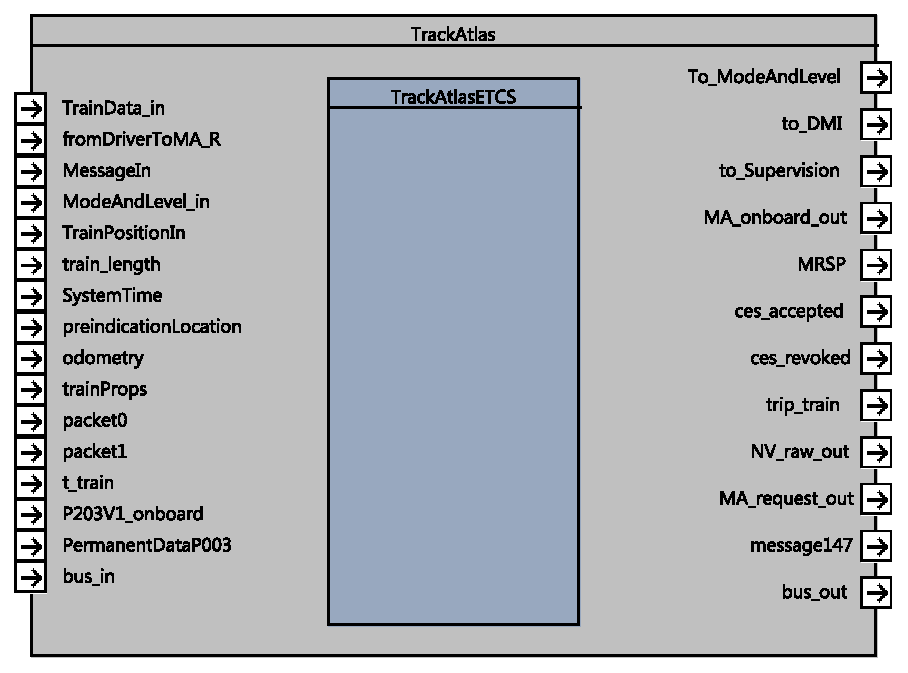
\includegraphics[width=.8\textwidth]{images/F2_4_TrackAtlas.pdf}
\caption{TrackAtlas component SysML diagram.}\label{f:manage_track_data_interface}
\end{figure}


\subsubsection{Inputs}\label{s:manage_track_data_inputs}

\paragraph{MessageIn}

\begin{longtable}{p{.25\textwidth}p{.7\textwidth}}
\toprule
Input name				& MessageIn \\
\midrule
Description				& Track to train message (as defined in Subset 026, chapter 8) with containing packets (as defined in Subset 026, chapter 7) \\
\midrule
Source					& F2.1 Manage\_TracksideInformation\_Integration\\ 
\midrule
Type					& Common\_Types\_Pkg::ReceivedMessage\_T \\
\midrule
Valid range of values	& valid combinations of Messages and Packets as implemented in the package TrackMessages \\
\midrule
Behaviour when value is at boundary	& n/a\\
\midrule
Behaviour for values out of valid range	& Invalid messages/ packets are ignored. \\
\midrule
Behaviour when value is erroneous, absent or unwanted (i.e. spurious) & The messages are only seen as valid if they are present. \\
\bottomrule
\end{longtable}


\paragraph{ModeAndLevel\_in}

\begin{longtable}{p{.25\textwidth}p{.7\textwidth}}
\toprule
Input name				& ModeAndLevel\_in \\
\midrule
Description				& Status data on mode and level\\
\midrule
Source					& F2.5 ManageModeAndLevel \\ 
\midrule
Type					& Level\_And\_Mode\_Types\_Pkg::T\_Mode\_Level \\
\midrule
Valid range of values	& n/a, as this is a type based on enumerations which can not reach invalid state in SCADE \\
\midrule
Behaviour when value is at boundary	& n/a\\
\midrule
Behaviour for values out of valid range	& n/a\\
\midrule
Behaviour when value is erroneous, absent or unwanted (i.e. spurious) & n/a\\
\bottomrule
\end{longtable}

\paragraph{TrainData\_in}

\begin{longtable}{p{.25\textwidth}p{.7\textwidth}}
\toprule
Input name				& TrainData\_in\\
\midrule
Description				& Data received from TIU\\
\midrule
Source					& F2.3 trainData \\ 
\midrule
Type					& TrackAtlasTypes::FromTIU\_tl \\
\midrule
Valid range of values	& n/a\\
\midrule
Behaviour when value is at boundary	& n/a\\
\midrule
Behaviour for values out of valid range	& n/a\\
\midrule
Behaviour when value is erroneous, absent or unwanted (i.e. spurious) & n/a\\
\midrule
Remark & This input is unused at the moment\\

\bottomrule
\end{longtable}

\paragraph{TrainPositionIn}

\begin{longtable}{p{.25\textwidth}p{.7\textwidth}}
\toprule
Input name				& TrainPositionIn\\
\midrule
Description				& Structured Information about all aspects of the current state of the train with respect to the coordinate system, balise positioning and integrity information and the train position\\
\midrule
Source					& F2.6 calculateTrainPosition \\ 
\midrule
Type					& TrainPosition\_Types\_Pck::trainPosition\_T \\
\midrule
Valid range of values	& as defined by CalculateTrainPosition \\
\midrule
Behaviour when value is at boundary	& n/a\\
\midrule
Behaviour for values out of valid range	& n/a\\
\midrule
Behaviour when value is erroneous, absent or unwanted (i.e. spurious) & n/a\\
\bottomrule
\end{longtable}

\paragraph{train\_length}

\begin{longtable}{p{.25\textwidth}p{.7\textwidth}}
\toprule
Input name				& train\_length\\
\midrule
Description				& Train length\\
\midrule
Source					& TIU \\ 
\midrule
Type					& Obu\_BasicTypes\_Pkg::L\_internal\_Type\\
\midrule
Valid range of values	& not checked at the moment \\
\midrule
Behaviour when value is at boundary	& n/a\\
\midrule
Behaviour for values out of valid range	& n/a\\
\midrule
Behaviour when value is erroneous, absent or unwanted (i.e. spurious) & n/a\\
\midrule
Remark & This input shall be removed as soon as the input \emph{TrainData\_in} will be defined and used\\
\bottomrule


\end{longtable}

\paragraph{SystemTime}

\begin{longtable}{p{.25\textwidth}p{.7\textwidth}}
\toprule
Input name				& SystemTime\\
\midrule
Description				& Reference time of the EVC\\
\midrule
Source					& F2 input API\_SystemTime \\ 
\midrule
Type					& Obu\_BasicTypes\_Pkg::T\_internal\_Type\\
\midrule
Valid range of values	& n/a \\
\midrule
Behaviour when value is at boundary	& n/a\\
\midrule
Behaviour for values out of valid range	& n/a\\
\midrule
Behaviour when value is erroneous, absent or unwanted (i.e. spurious) & n/a\\

\bottomrule

\end{longtable}

\paragraph{preindicationLocation}

\begin{longtable}{p{.25\textwidth}p{.7\textwidth}}
\toprule
Input name				& preindicationLocation\\
\midrule
Description				& Preindication location for speed or target supervision \\
\midrule
Source					& F2.7 SpeedSupervision\_Integration \\ 
\midrule
Type					& Obu\_BasicTypes\_Pkg::L\_internal\_Type\\
\midrule
Valid range of values	& n/a \\
\midrule
Behaviour when value is at boundary	& n/a\\
\midrule
Behaviour for values out of valid range	& n/a\\
\midrule
Behaviour when value is erroneous, absent or unwanted (i.e. spurious) & n/a\\

\bottomrule


\end{longtable}

\paragraph{odometry}

\begin{longtable}{p{.25\textwidth}p{.7\textwidth}}
\toprule
Input name				& odometry\\
\midrule
Description				& Odometry Data  \\
\midrule
Source					& F2 input API\_Odometry \\ 
\midrule
Type					& Obu\_BasicTypes\_Pkg::odometry\_T\\
\midrule
Valid range of values	& n/a \\
\midrule
Behaviour when value is at boundary	& n/a\\
\midrule
Behaviour for values out of valid range	& n/a\\
\midrule
Behaviour when value is erroneous, absent or unwanted (i.e. spurious) & n/a\\

\bottomrule


\end{longtable}

\paragraph{fromDriverToMA\_R}

\begin{longtable}{p{.25\textwidth}p{.7\textwidth}}
\toprule
Input name				& fromDriverToMA\_R\\
\midrule
Description				& Data sent from DMI to MA Request function  \\
\midrule
Source					& DMI interface \\ 
\midrule
Type					& MA\_Request::Driver2MAR\_T\\
\midrule
Valid range of values	& n/a \\
\midrule
Behaviour when value is at boundary	& n/a\\
\midrule
Behaviour for values out of valid range	& n/a\\
\midrule
Behaviour when value is erroneous, absent or unwanted (i.e. spurious) & n/a\\

\bottomrule


\end{longtable}

\paragraph{trainProps}

\begin{longtable}{p{.25\textwidth}p{.7\textwidth}}
\toprule
Input name				& trainProps\\
\midrule
Description				& Train Characteristics as provided by CalculateTrainPosition  \\
\midrule
Source					& F2.3 trainData\newline
F2.10 manageDMI\_Input \\ 
\midrule
Type					& TrainPosition\_Types\_Pck::trainProperties\_T\\
\midrule
Valid range of values	& n/a \\
\midrule
Behaviour when value is at boundary	& n/a\\
\midrule
Behaviour for values out of valid range	& n/a\\
\midrule
Behaviour when value is erroneous, absent or unwanted (i.e. spurious) & n/a\\

\bottomrule


\end{longtable}

\paragraph{packet0}

\begin{longtable}{p{.25\textwidth}p{.7\textwidth}}
\toprule
Input name				& packet0\\
\midrule
Description				& Train Position Report packet 0  \\
\midrule
Source					& F2.8 ProvidePositionReport \\ 
\midrule
Type					& Packet\_TrainTypes\_Pkg::PT0\_PositionReport\_T\\
\midrule
Valid range of values	& n/a \\
\midrule
Behaviour when value is at boundary	& n/a\\
\midrule
Behaviour for values out of valid range	& n/a\\
\midrule
Behaviour when value is erroneous, absent or unwanted (i.e. spurious) & n/a\\

\bottomrule


\end{longtable}

\paragraph{packet1}

\begin{longtable}{p{.25\textwidth}p{.7\textwidth}}
\toprule
Input name				& packet1\\
\midrule
Description				& Train Position Report based on two balise groups (Packet 1)  \\
\midrule
Source					& F2.8 ProvidePositionReport \\ 
\midrule
Type					& Packet\_TrainTypes\_Pkg::PT1\_PositionReport\_2BG\_T\\
\midrule
Valid range of values	& n/a \\
\midrule
Behaviour when value is at boundary	& n/a\\
\midrule
Behaviour for values out of valid range	& n/a\\
\midrule
Behaviour when value is erroneous, absent or unwanted (i.e. spurious) & n/a\\

\bottomrule


\end{longtable}


\paragraph{t\_train}

\begin{longtable}{p{.25\textwidth}p{.7\textwidth}}
\toprule
Input name				& t\_train\\
\midrule
Description				& Time reference of the EVC  \\
\midrule
Source					& F2 input API\_SystemTime\\ 
\midrule
Type					& T\_TRAIN\\
\midrule
Valid range of values	& n/a \\
\midrule
Behaviour when value is at boundary	& n/a\\
\midrule
Behaviour for values out of valid range	& n/a\\
\midrule
Behaviour when value is erroneous, absent or unwanted (i.e. spurious) & n/a\\

\bottomrule


\end{longtable}


\paragraph{bus\_in}

\begin{longtable}{p{.25\textwidth}p{.7\textwidth}}
\toprule
Input name				& bus\_in\\
\midrule
Description				& Train to track message bus  \\
\midrule
Source					& F2.3 trainData\\ 
\midrule
Type					& TM\_TrainTrack\_Bus::M\_TrainTrackMessageBus\_t\\
\midrule
Valid range of values	& n/a \\
\midrule
Behaviour when value is at boundary	& n/a\\
\midrule
Behaviour for values out of valid range	& n/a\\
\midrule
Behaviour when value is erroneous, absent or unwanted (i.e. spurious) & n/a\\

\bottomrule


\end{longtable}




\paragraph{P203V1\_onboard}

\begin{longtable}{p{.25\textwidth}p{.7\textwidth}}
\toprule
Input name				& P203V1\_onboard\\
\midrule
Description				& Default values for track to train packet 203 as stored onboard. In case of a baseline 2 track, these data are used to build a baseline 3- conformal packet 3. \\
\midrule
Source					& F2 input API\_persistentData\\ 
\midrule
Type					& TM\_baseline2::P203V1\_OBU\_T\\
\midrule
Valid range of values	& n/a \\
\midrule
Behaviour when value is at boundary	& n/a\\
\midrule
Behaviour for values out of valid range	& n/a\\
\midrule
Behaviour when value is erroneous, absent or unwanted (i.e. spurious) & n/a\\

\bottomrule


\end{longtable}

\paragraph{PermanentDataP003}

\begin{longtable}{p{.25\textwidth}p{.7\textwidth}}
\toprule
Input name				& PermanentDataP003\\
\midrule
Description				& Default values for track to train packet 3 (baseline 2) as stored onboard. In case of a baseline 2 track, these data are used to build a baseline 3- conformal packet 3. \\
\midrule
Source					& F2 input API\_persistentData\\ 
\midrule
Type					& TM\_baseline2::P003\_permanent\_data\_T\\
\midrule
Valid range of values	& n/a \\
\midrule
Behaviour when value is at boundary	& n/a\\
\midrule
Behaviour for values out of valid range	& n/a\\
\midrule
Behaviour when value is erroneous, absent or unwanted (i.e. spurious) & n/a\\

\bottomrule


\end{longtable}


\subsubsection{Outputs}\label{s:manage_track_data_outputs}

\paragraph{NV\_raw\_out}

\begin{longtable}{p{.25\textwidth}p{.7\textwidth}}
\toprule
Output name				& NV\_raw\_out \\
\midrule
Description				& National values as received from the track (in case of a baseline 3 trackside, or national values as calculated by TrackAtlas (in case of reception of a baseline 2 trackside) \\
\midrule
Destination				& Various recipients: SDM, Mode and Levels\\ 
\midrule
Type					& TM::P003\_OBU\_T \\
\midrule
Valid range of values	& n/a \\
\midrule
Behaviour when value is at boundary	& n/a  \\
\midrule
Behaviour for values out of valid range	& n/a  \\
\midrule
Behaviour when value is erroneous, absent or unwanted (i.e. spurious) & n/a  \\
\bottomrule
\end{longtable}


\paragraph{To\_ModeAndLevel}

\begin{longtable}{p{.25\textwidth}p{.7\textwidth}}
\toprule
Output name				& To\_ModeAndLevel \\
\midrule
Description				& Aggregated status information concerning the data maintained by TrackAtlas, for usage by Mode and Levels Management Module \\
\midrule
Destination				& F2.5 ManageLevelAndMode \\ 
\midrule
Type					& TrackAtlasTypes::DataForModeAndLevel\_t\\
\midrule
Valid range of values	& n/a \\
\midrule
Behaviour when value is at boundary	& n/a  \\
\midrule
Behaviour for values out of valid range	& n/a  \\
\midrule
Behaviour when value is erroneous, absent or unwanted (i.e. spurious) & n/a  \\
\bottomrule
\end{longtable}

\paragraph{to\_DMI}

\begin{longtable}{p{.25\textwidth}p{.7\textwidth}}
\toprule
Output name				& to\_DMI \\
\midrule
Description				& Aggregated information concerning Movement Authority (MA information, Gradient Profile Information, MRSP information; formatted for use by DMI \\
\midrule
Destination				& F2.11 manageDMI\_Output  \\ 
\midrule
Type					& TrackAtlasTypes::DataForDMI\_t\\
\midrule
Valid range of values	& n/a \\
\midrule
Behaviour when value is at boundary	& n/a  \\
\midrule
Behaviour for values out of valid range	& n/a  \\
\midrule
Behaviour when value is erroneous, absent or unwanted (i.e. spurious) & n/a  \\
\bottomrule
\end{longtable}

\paragraph{MRSP}

\begin{longtable}{p{.25\textwidth}p{.7\textwidth}}
\toprule
Output name				& MRSP \\
\midrule
Description				& Aggregated information concerning Movement Authority (MA information, Gradient Profile Information, MRSP information; formatted for use by SDM. \\
\midrule
Destination				& Output is currently not used in the model.  \\ 
\midrule
Type					& TrackAtlasTypes::DataForSupervision\_nextGen\_t\\
\midrule
Valid range of values	& n/a \\
\midrule
Behaviour when value is at boundary	& n/a  \\
\midrule
Behaviour for values out of valid range	& n/a  \\
\midrule
Behaviour when value is erroneous, absent or unwanted (i.e. spurious) & n/a  \\
\bottomrule
\end{longtable}

\paragraph{to\_Supervision}

\begin{longtable}{p{.25\textwidth}p{.7\textwidth}}
\toprule
Output name				& to\_Supervision \\
\midrule
Description				& Most restrictive speed profile \\
\midrule
Destination				&F2.7 SpeedSupervision\_Integration  \\ 
\midrule
Type					& TrackAtlasTypes::MRSP\_Profile\_t\\
\midrule
Valid range of values	& n/a \\
\midrule
Behaviour when value is at boundary	& n/a  \\
\midrule
Behaviour for values out of valid range	& n/a  \\
\midrule
Behaviour when value is erroneous, absent or unwanted (i.e. spurious) & n/a  \\
\bottomrule
\end{longtable}

\paragraph{MA\_onboard\_out}

\begin{longtable}{p{.25\textwidth}p{.7\textwidth}}
\toprule
Output name				& MA\_onboard\_out \\
\midrule
Description				& Movement authority information extracted from Packet 15 or 16, normalised to train coordinate system\\
\midrule
Destination				& Output is currently not used in the model.  \\ 
\midrule
Type					& TrackAtlasTypes::MovementAuthority\_t\\
\midrule
Valid range of values	& n/a \\
\midrule
Behaviour when value is at boundary	& n/a  \\
\midrule
Behaviour for values out of valid range	& n/a  \\
\midrule
Behaviour when value is erroneous, absent or unwanted (i.e. spurious) & n/a  \\
\bottomrule
\end{longtable}

\paragraph{bus\_out}

\begin{longtable}{p{.25\textwidth}p{.7\textwidth}}
\toprule
Output name				& bus\_out \\
\midrule
Description				& Train to track message bus containing train to track messages with optional packets \\
\midrule
Destination				& F2.8 ProvidePositionReport  \\ 
\midrule
Type					& TM\_TrainTrack\_Bus::M\_TrainTrackMessageBus\_t\\
\midrule
Valid range of values	& n/a \\
\midrule
Behaviour when value is at boundary	& n/a  \\
\midrule
Behaviour for values out of valid range	& n/a  \\
\midrule
Behaviour when value is erroneous, absent or unwanted (i.e. spurious) & n/a  \\
\bottomrule
\end{longtable}

\paragraph{ces\_accepted}

\begin{longtable}{p{.25\textwidth}p{.7\textwidth}}
\toprule
Output name				& ces\_accepted \\
\midrule
Description				& Flag to indicate that a conditional emergency stop has been accepted in the current cycle \\
\midrule
Destination				& Output is currently not used in the model.  \\ 
\midrule
Type					& bool\\
\midrule
Valid range of values	& true/ false \\
\midrule
Behaviour when value is at boundary	& n/a  \\
\midrule
Behaviour for values out of valid range	& n/a  \\
\midrule
Behaviour when value is erroneous, absent or unwanted (i.e. spurious) & n/a  \\
\bottomrule
\end{longtable}

\paragraph{ces\_revoked}

\begin{longtable}{p{.25\textwidth}p{.7\textwidth}}
\toprule
Output name				& ces\_revoked \\
\midrule
Description				& Flag to indicate that a conditional emergency stop has been revoked in the current cycle \\
\midrule
Destination				& Output is currently not used in the model.  \\ 
\midrule
Type					& bool\\
\midrule
Valid range of values	& true/ false \\
\midrule
Behaviour when value is at boundary	& n/a  \\
\midrule
Behaviour for values out of valid range	& n/a  \\
\midrule
Behaviour when value is erroneous, absent or unwanted (i.e. spurious) & n/a  \\
\bottomrule
\end{longtable}

\paragraph{trip\_train}

\begin{longtable}{p{.25\textwidth}p{.7\textwidth}}
\toprule
Output name				& trip\_train \\
\midrule
Description				& Flag to indicate that the train must be tripped \\
\midrule
Destination				& Output is currently not used in the model.\\ 
\midrule
Type					& bool\\
\midrule
Valid range of values	& true/ false \\
\midrule
Behaviour when value is at boundary	& n/a  \\
\midrule
Behaviour for values out of valid range	& n/a  \\
\midrule
Behaviour when value is erroneous, absent or unwanted (i.e. spurious) & n/a  \\
\bottomrule
\end{longtable}


\subsection{Subcomponents}\label{s:manage_track_data_subcomponents}

\subsubsection{StoreRaw\_NV}
%set the master document for easy compilation
%!TEX root = ../D3_5_3.tex

\paragraph{Component Requirements}

\begin{longtable}{p{.25\textwidth}p{.7\textwidth}}
\toprule
Component name			& StoreRaw\_NV \\
\midrule
Link to SCADE model		& {\footnotesize \url{https://github.com/openETCS/modeling/tree/master/model/Scade/
System/ObuFunctions/TrackAtlas/TA\_Storage}} \\
\midrule
SCADE designer			& Jakob G\"artner, LEA Railergy \\
\midrule
Description				& Receives National Values from the track. Stores them "as-is" onboard. If Subset\_026 chapter 6 is applicable, baseline 3 conformal information is calculated based on packet 3 and packet 203 (according to older versions). Missing trackside information is complemented throug default onboard values. \\
\midrule
Input documents	& 
Subset-026, Chapter 6
Subset-026, Chapter 7
Subset-026, Chapter 8\\
\midrule
Safety integrity level	& 4 \\
\midrule
Time constraints		& n/a \\
\midrule
API requirements 		& Based on data formats and functions defined by TrackMessages package\\
\bottomrule
\end{longtable}


\paragraph{Interface}

For an overview of the interface of this internal component we refer to the SCADE model (cf.~link above) respectively the SCADE generated documentation.

\subsubsection{Build\_GradientProfile}
%set the master document for easy compilation
%!TEX root = ../D3_5_3.tex

\paragraph{Component Requirements}

\begin{longtable}{p{.25\textwidth}p{.7\textwidth}}
\toprule
Component name			& Build\_GradientProfile \\
\midrule
Link to SCADE model		& {\footnotesize \url{https://github.com/openETCS/modeling/tree/master/model/Scade/
System/ObuFunctions/TrackAtlas/TA\_Gradient.xscade}} \\
\midrule
SCADE designer			& Jakob G\"artner, LEA Railergy  \\
\midrule
Description				& Receives Track to Train Packet 21 (Gradient Profile). References the data to the train coordinate system. Converts incremental distances to absolute distances in the train's coordinate system. Merges the information from sequentially received packets into a continuous Gradient Profile. Truncates the profile as required\\
\midrule
Input documents	& 
Subset-026, Chapter 3.11.12\newline
Subset-026, Chapter 7\\

\midrule
Safety integrity level	& 4 \\
\midrule
Time constraints		& n/a\\
\midrule
API requirements 		& n/a \\
\bottomrule
\end{longtable}


\paragraph{Interface}

For an overview of the interface of this internal component we refer to the SCADE model (cf.~link above) respectively the SCADE generated documentation.

\subsubsection{Build\_MA}
%set the master document for easy compilation
%!TEX root = ../D3_5_3.tex

\paragraph{Component Requirements}

\begin{longtable}{p{.25\textwidth}p{.7\textwidth}}
\toprule
Component name			& Build\_MA \\
\midrule
Link to SCADE model		& {\footnotesize \url{http://???}} \\
\midrule
SCADE designer			& Jakob G\"artner, LEA \\
\midrule
Description				& [Brief description of functionality] \\
\midrule
Input documents	& 
Subset-026, Chapter ?.?\newline
Subset-026, Chapter ?.?\newline
Subset-026, Chapter ?.?.?\\
\midrule
Safety integrity level	& 4 \\
\midrule
Time constraints		& [If applicable description of time constraints, otherwise n/a] \\
\midrule
API requirements 		& [If applicable description of API requirements, otherwise n/a] \\
\bottomrule
\end{longtable}


\paragraph{Interface}

For an overview of the interface of this internal component we refer to the SCADE model (cf.~link above) respectively the SCADE generated documentation.

\subsubsection{Build\_MRSP}
%set the master document for easy compilation
%!TEX root = ../D3_5_3.tex

\paragraph{Component Requirements}

\begin{longtable}{p{.25\textwidth}p{.7\textwidth}}
\toprule
Component name			& Build\_MRSP \\
\midrule
Link to SCADE model		& {\footnotesize \url{https://github.com/openETCS/modeling/tree/master/model/Scade/
System/ObuFunctions/TrackAtlas/TA\_MRSP}} \\
\midrule
SCADE designer			& Jakob G\"artner, LEA \\
\midrule
Description				& Reduces the various Speed Profiles to Most Restrictive Speed Profile information \\
\midrule
Input documents	& 
Subset-026, Chapter 3.11\\
\midrule
Safety integrity level	& 4 \\
\midrule
Time constraints		& n/a \\
\midrule
API requirements 		& n/a \\
\bottomrule
\end{longtable}


\paragraph{Interface}

For an overview of the interface of this internal component we refer to the SCADE model (cf.~link above) respectively the SCADE generated documentation.

\subsubsection{Manage\_EmergencyStop}
%set the master document for easy compilation
%!TEX root = ../D3_5_3.tex

\paragraph{Component Requirements}

\begin{longtable}{p{.25\textwidth}p{.7\textwidth}}
\toprule
Component name			& Manage\_EmergencyStop \\
\midrule
Link to SCADE model		& {\footnotesize \url{https://github.com/openETCS/modeling/tree/master/model/Scade/
System/ObuFunctions/TrackAtlas/TA\_EmergencyS_top.xscade}} \\
\midrule
SCADE designer			& Johannes Kastner, ICS AG; Jakob G\"artner, LEA Railergy\\
\midrule
Description				& Manages Emergency Stop Messages\\
\midrule
Input documents	& 
Subset-026, Chapter 3\\
\midrule
Safety integrity level	& 4 \\
\midrule
Time constraints		& n/a \\
\midrule
API requirements 		& n/a \\
\bottomrule
\end{longtable}


\paragraph{Interface}

For an overview of the interface of this internal component we refer to the SCADE model (cf.~link above) respectively the SCADE generated documentation.

\subsubsection{Manage\_MA\_Request}
%set the master document for easy compilation
%!TEX root = ../D3_5_3.tex

\paragraph{Component Requirements}

\begin{longtable}{p{.25\textwidth}p{.7\textwidth}}
\toprule
Component name			& Manage\_MA\_Request \\
\midrule
Link to SCADE model		& {\footnotesize \url{https://github.com/openETCS/modeling/tree/master/model/Scade/
System/ObuFunctions/TrackAtlas/TA\_MA\_Request}} \\
\midrule
SCADE designer			& Christian Stahl, TWT GmbH \\
\midrule
Description				& Manages reception of MA request parameters and sends MA request as specified\\
\midrule
Input documents	& 
Subset-026, Chapter ?.?\newline
Subset-026, Chapter ?.?\newline
Subset-026, Chapter ?.?.?\\
\midrule
Safety integrity level	& 4 \\
\midrule
Time constraints		& n/a \\
\midrule
API requirements 		& n/a]\\
\bottomrule
\end{longtable}


\paragraph{Interface}

For an overview of the interface of this internal component we refer to the SCADE model (cf.~link above) respectively the SCADE generated documentation.

\

